\scanpage{11}
\mspage{8}
Prouvons (iv). Supposons prouvé
\[
\pi_{j\alpha}\in\mathcal E\quad\text{pour}\quad j\notin[i,2n-i]
\tag{6.7}
\]
où $i\leq n$, et prouvons que
\deleted{\[\pi_{j\alpha}\in\mathcal E\quad\text{pour}\quad j\unsure{\in}\]}
\[
\pi_{j\alpha}\in\mathcal E\quad\text{pour }j=i\text{ ou }j=2n-i,
\tag{6.7'}
\]
ce qui prouvera (iv) \inserted{\figure{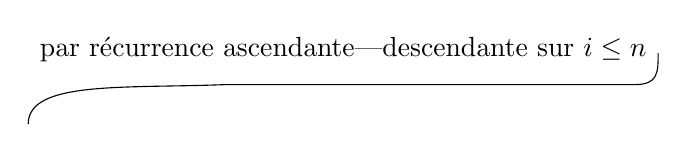
\begin{tikzpicture}[x=1cm,y=1cm]
\node at (0,.25) {par récurrence \unsure{ascendante|descendante} sur $i\leq n$};
\draw (-4,-.7) .. controls (-4,-.15) and (-2.8,-.25) .. (-1.5,-.2) -- (3.7,-.2) .. controls (4,-.2) and (4,-.05) .. (4,.2);
\end{tikzpicture}}}. Pour prouver $6.8.$ on procède par récurrence \deleted{\unsure{sur}} descendante sur $\alpha$, en supposant que
\[
\deleted{\unsure{\pi_{j\alpha}}}\quad\pi_{i,\alpha'}\in\mathcal E,\quad\pi_{2n-i,\alpha'}\in\mathcal E\quad\text{si }\alpha'>\alpha,
\tag{6.8}
\]
et on en conclura que
\[
\pi_{i,\alpha}\in\mathcal E,\quad\pi_{2n-i,\alpha}\in\mathcal E.
\tag{6.8'}
\]
\deleted{\unsure{Car|Cela} \deleted{doit} prouvera bien $(6.7')$, puisque on peut démarrer la récurrence ($\pi_{i,\alpha}=\pi_{2n-i,\alpha}=0$ si $\alpha$ grand). Si $\alpha=0$, on gagne grâce à la relation
\[
\sum_\alpha\pi_{i,\alpha}=\pi_i\quad\text{donc}\quad\pi_{i,0}=\pi_i-\sum_{\alpha\geq1}\pi_{i\alpha},
\tag{6.9}
\]
donc il suffit d'envisager le cas $\alpha\geq1$.}

Posons
\[
q_{i,\alpha}=1-\sum_{\alpha'>\alpha}\pi_{i,\alpha'}=\sum_{\alpha'\leq\alpha}\pi_{i,\unsure{\alpha|\alpha'}}
\]
donc grâce à $(6.8)$ on a
\[
q_{i,\alpha}\in\mathcal E\quad\deleted{\unsure{\mathcal E}}
\]
\mspage{10}
